\subsubsection{Exceptions in the 5-stage pipeline}

Asynchronous \textbf{interrupts can occur at any stage of the pipeline}. In the following figure we can see some examples of exceptions that can occur at any stage.
\begin{figure}[!htp]
    \centering
    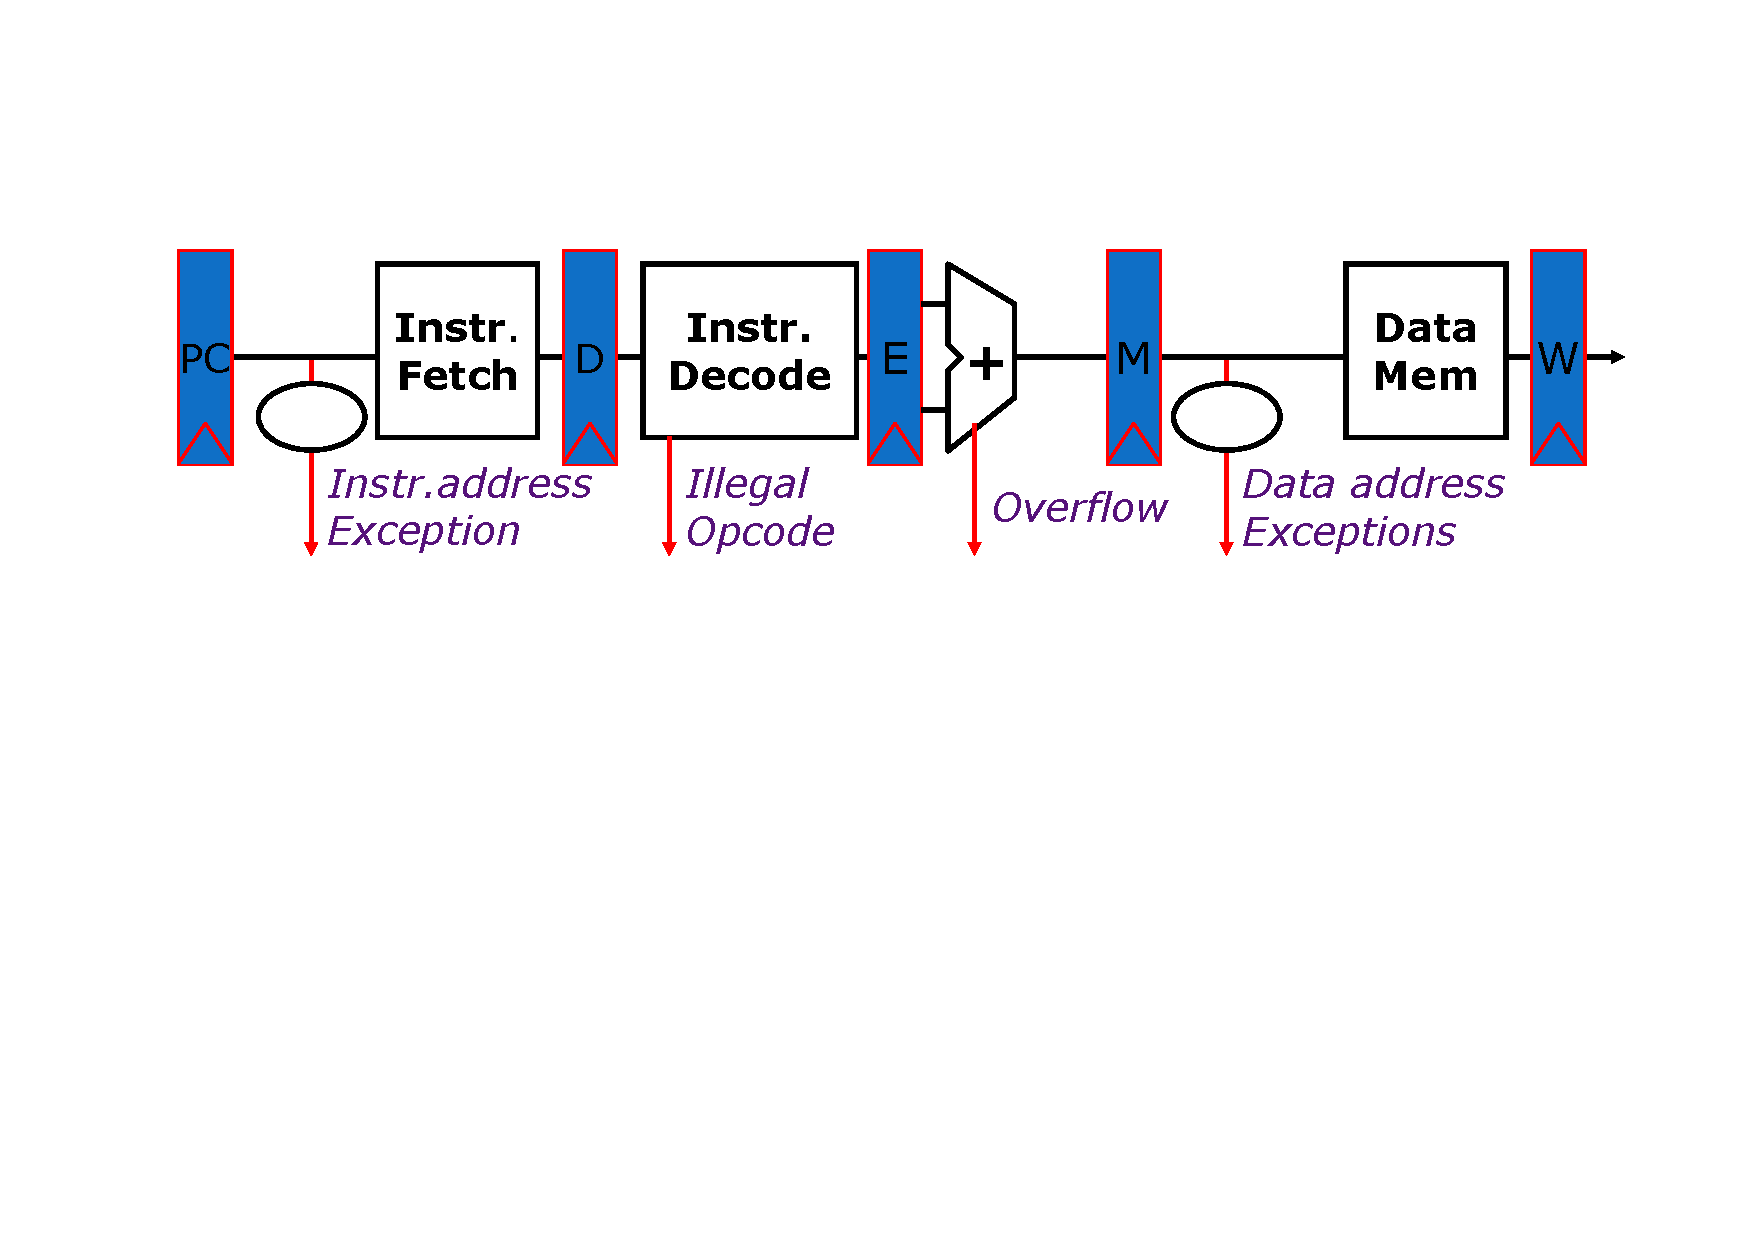
\includegraphics[width=.9\textwidth]{img/exceptions-in-the-5-stage-pipeline-1.pdf}
    \caption{\example{Example} of exceptions in the 5-stage pipeline.}
\end{figure}

\noindent
The aim of this section is to understand how to handle multiple simultaneous exceptions at different stages of the pipeline, and how and where to handle external asynchronous interrupts such as an I/O service request.

\begin{examplebox}[: Data Page Fault and Arithmetic Exception]
    In this first example of an exception in a 5-stage pipeline, we can see that pipelining can cause exceptions to be thrown \textbf{out of order}. In fact, we remember that exceptions can occur at different stages in the pipeline for different instructions.

    \highspace
    For example, a \textbf{Data Page Fault} occurs at the memory stage of the first instruction. The \textbf{Arithmetic Exception} occurs in the execution phase of the second instruction.

    Because of the pipelined execution, \textbf{the page fault occurs at the same time as the overflow}. Note, however, that the \textbf{data page fault MUST be handled first}.

    \begin{center}
        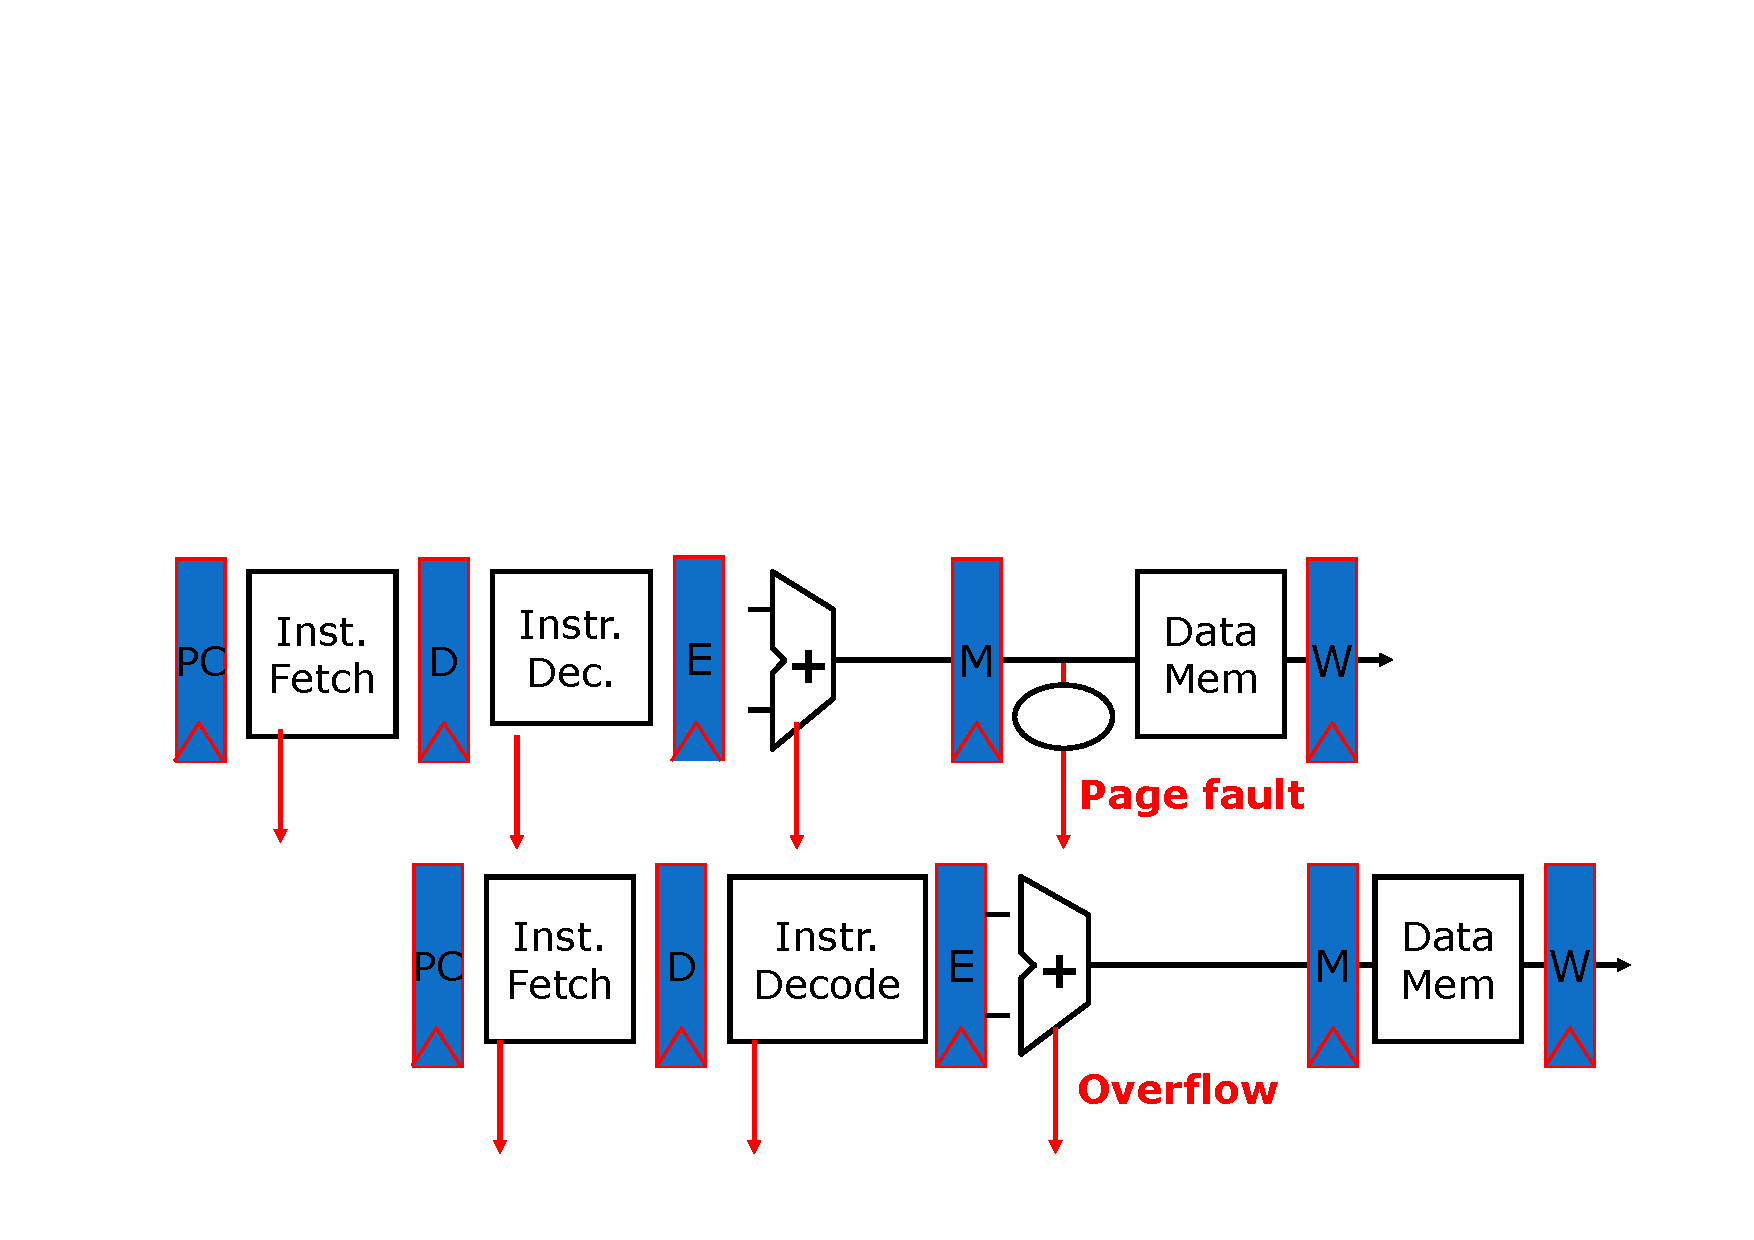
\includegraphics[width=\textwidth]{img/exceptions-in-the-5-stage-pipeline-2.pdf}
    \end{center}
\end{examplebox}

\newpage

\begin{examplebox}[: Instruction Page Fault and Data Page Fault]
    The exceptions may not always be as waterfall. As we said in the first example, the exceptions can be thrown out of order.

    \highspace
    In this case we have an \textbf{Instruction Page Fault} that occurs in the \textbf{Instruction Memory} stage of the second instruction. There is also a \textbf{Data Page Fault} in the memory phase of the first instruction.

    Despite the first example, \textbf{the instruction page fault is handled first!}

    \begin{center}
        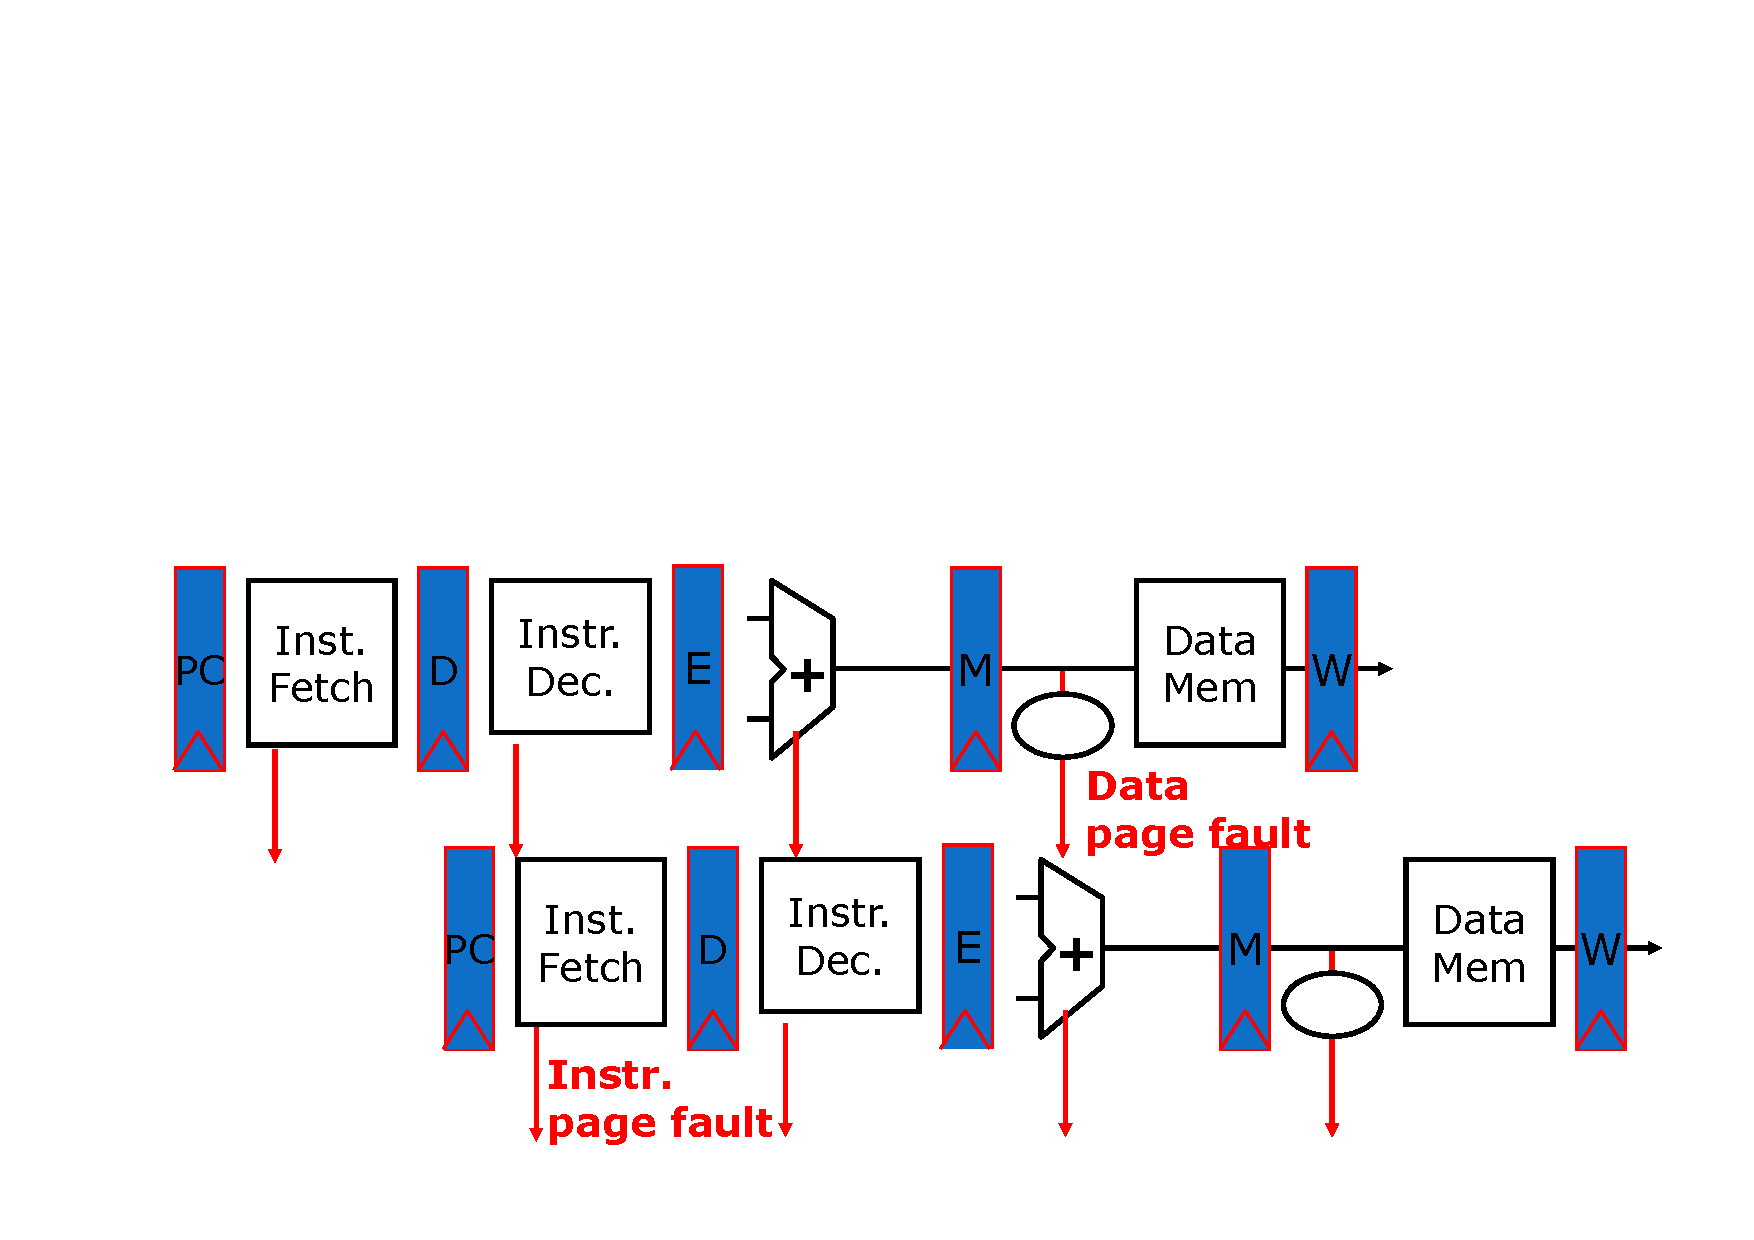
\includegraphics[width=\textwidth]{img/exceptions-in-the-5-stage-pipeline-3.pdf}
    \end{center}
\end{examplebox}

\noindent
From the previous examples, we know that out-of-order is a serious pipelining problem.

\begin{flushleft}
    \textcolor{Green4}{\faIcon{check} \textbf{How can the pipeline be modified to solve these problems?}}
\end{flushleft}
By using the exception flag and the PC.
\begin{enumerate}
    \item First, hold the \textbf{exception flag} and \textbf{pass it through the pipeline}.
    
    \item Hold the \textbf{Program Counter} (PC) and \textbf{pass it through the pipeline} (to be saved and restored after the Exception Handler Routine).
    
    \item Finally, do \textbf{not react to the exception until it reaches the commit point}. In other words, wait until the end of MEM stage to raise the exception. 
\end{enumerate}
Please note that \textbf{when the instruction reaches the Commit Point}, before entering the Write Back (WB) phase, the \textbf{following steps are performed}:
\begin{itemize}
    \item Store the Program Counter in the Exception Program Counter ($\textbf{\texttt{PC}} \boldsymbol{\rightarrow} \textbf{\texttt{EPC}}$) and store the Interrupt Handler Address in the Program Counter ($\textbf{\texttt{IHA}} \boldsymbol{\rightarrow} \textbf{\texttt{PC}}$).
    
    \item Make all \textbf{next instructions in previous stages \texttt{NOP} operations} (see Figure \ref{fig: instruction reaches the commit point} on page \pageref{fig: instruction reaches the commit point}).
    
    \item \textbf{Handle interrupts} by \dquotes{faulting nop} in the \textbf{Instruction Fetch (IF) stage}.
\end{itemize}
At the end of the Exception Handler Routine, the instruction is re-executed.

\highspace
By adopting this solution, all \textbf{exceptions are deferred to be handled in order at the MEM stage}, as in any non-pipelined processor.

\newpage

\begin{figure}[!htp]
    \centering
    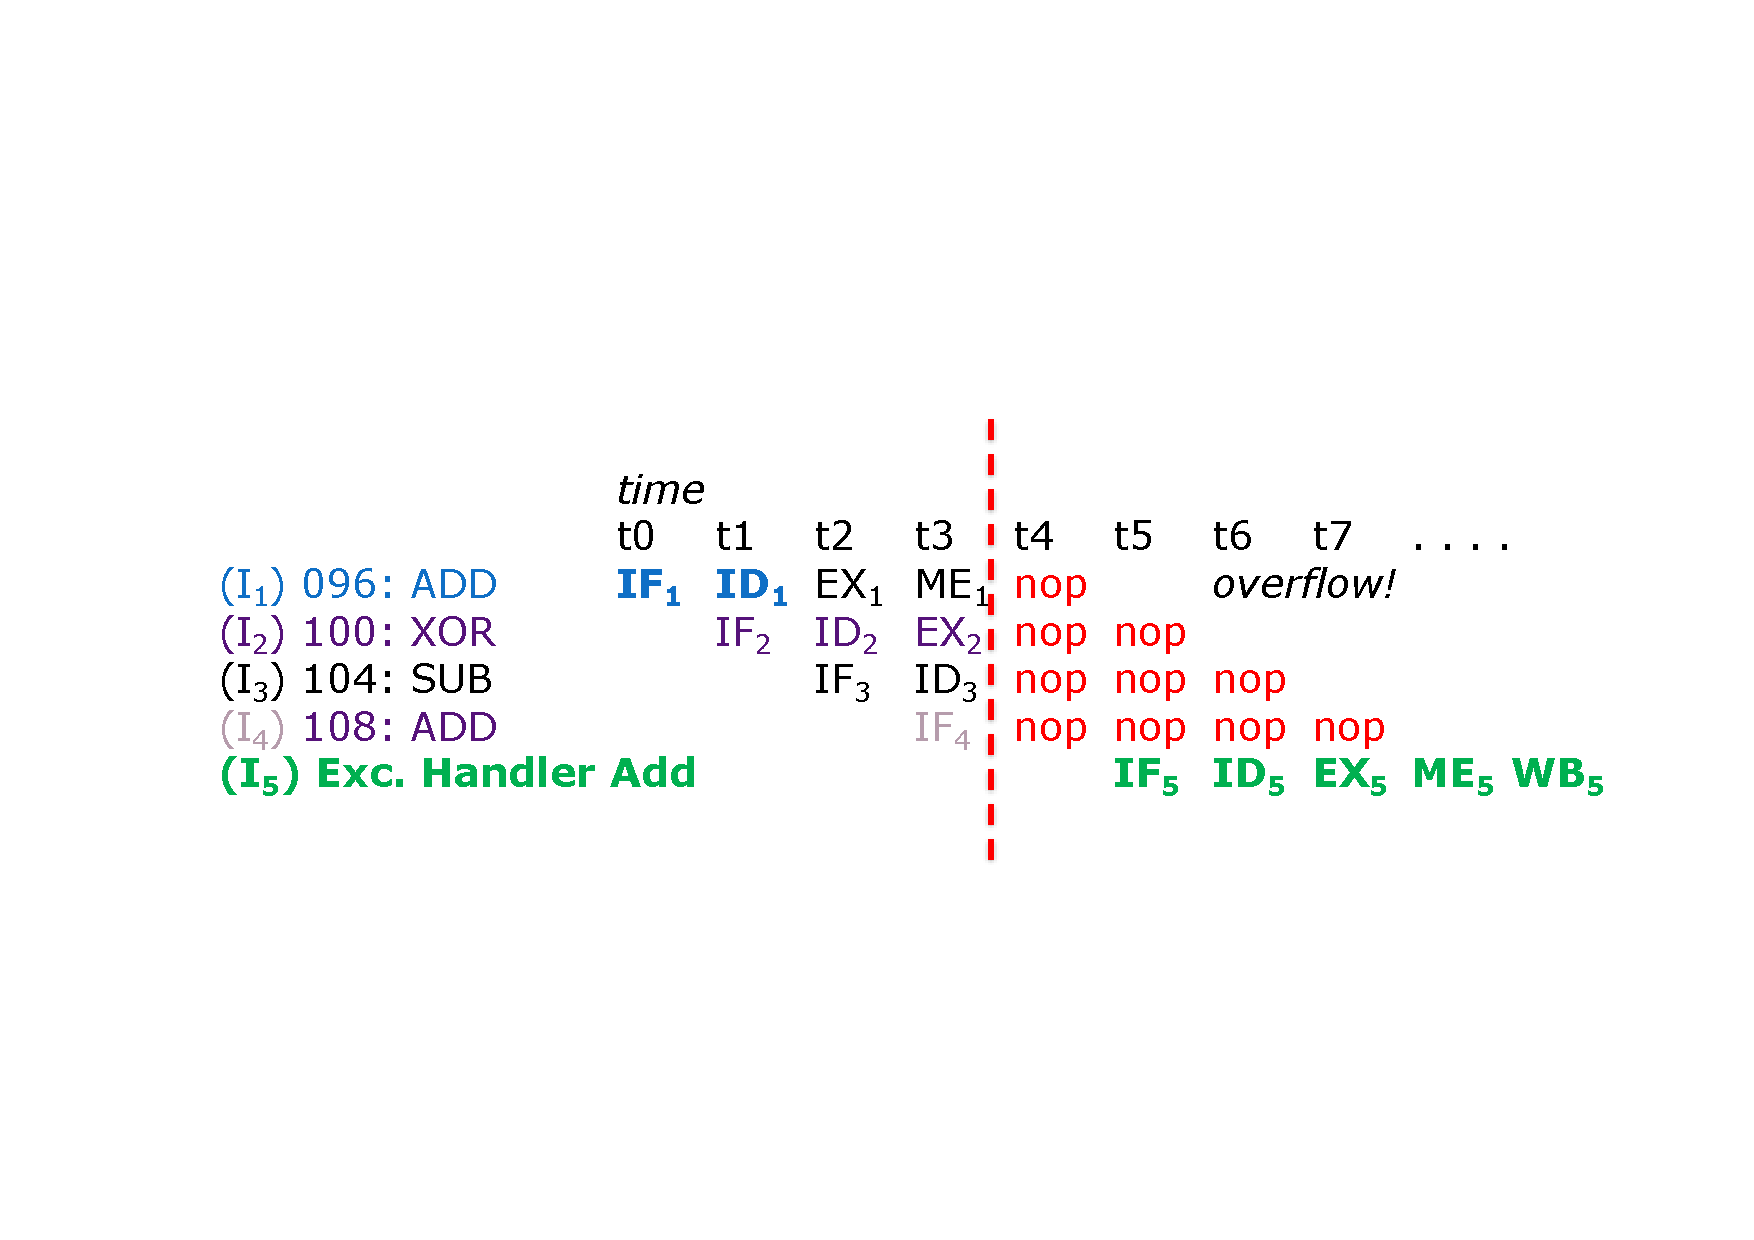
\includegraphics[width=\textwidth]{img/exceptions-in-the-5-stage-pipeline-4.pdf}
    \caption{Make all next instructions in previous stage NOP operations.}
    \label{fig: instruction reaches the commit point}
\end{figure}

\noindent
In the following figure, we can see how the execution flow changes when an exception occurs in a pipeline.

\begin{figure}[!htp]
    \centering
    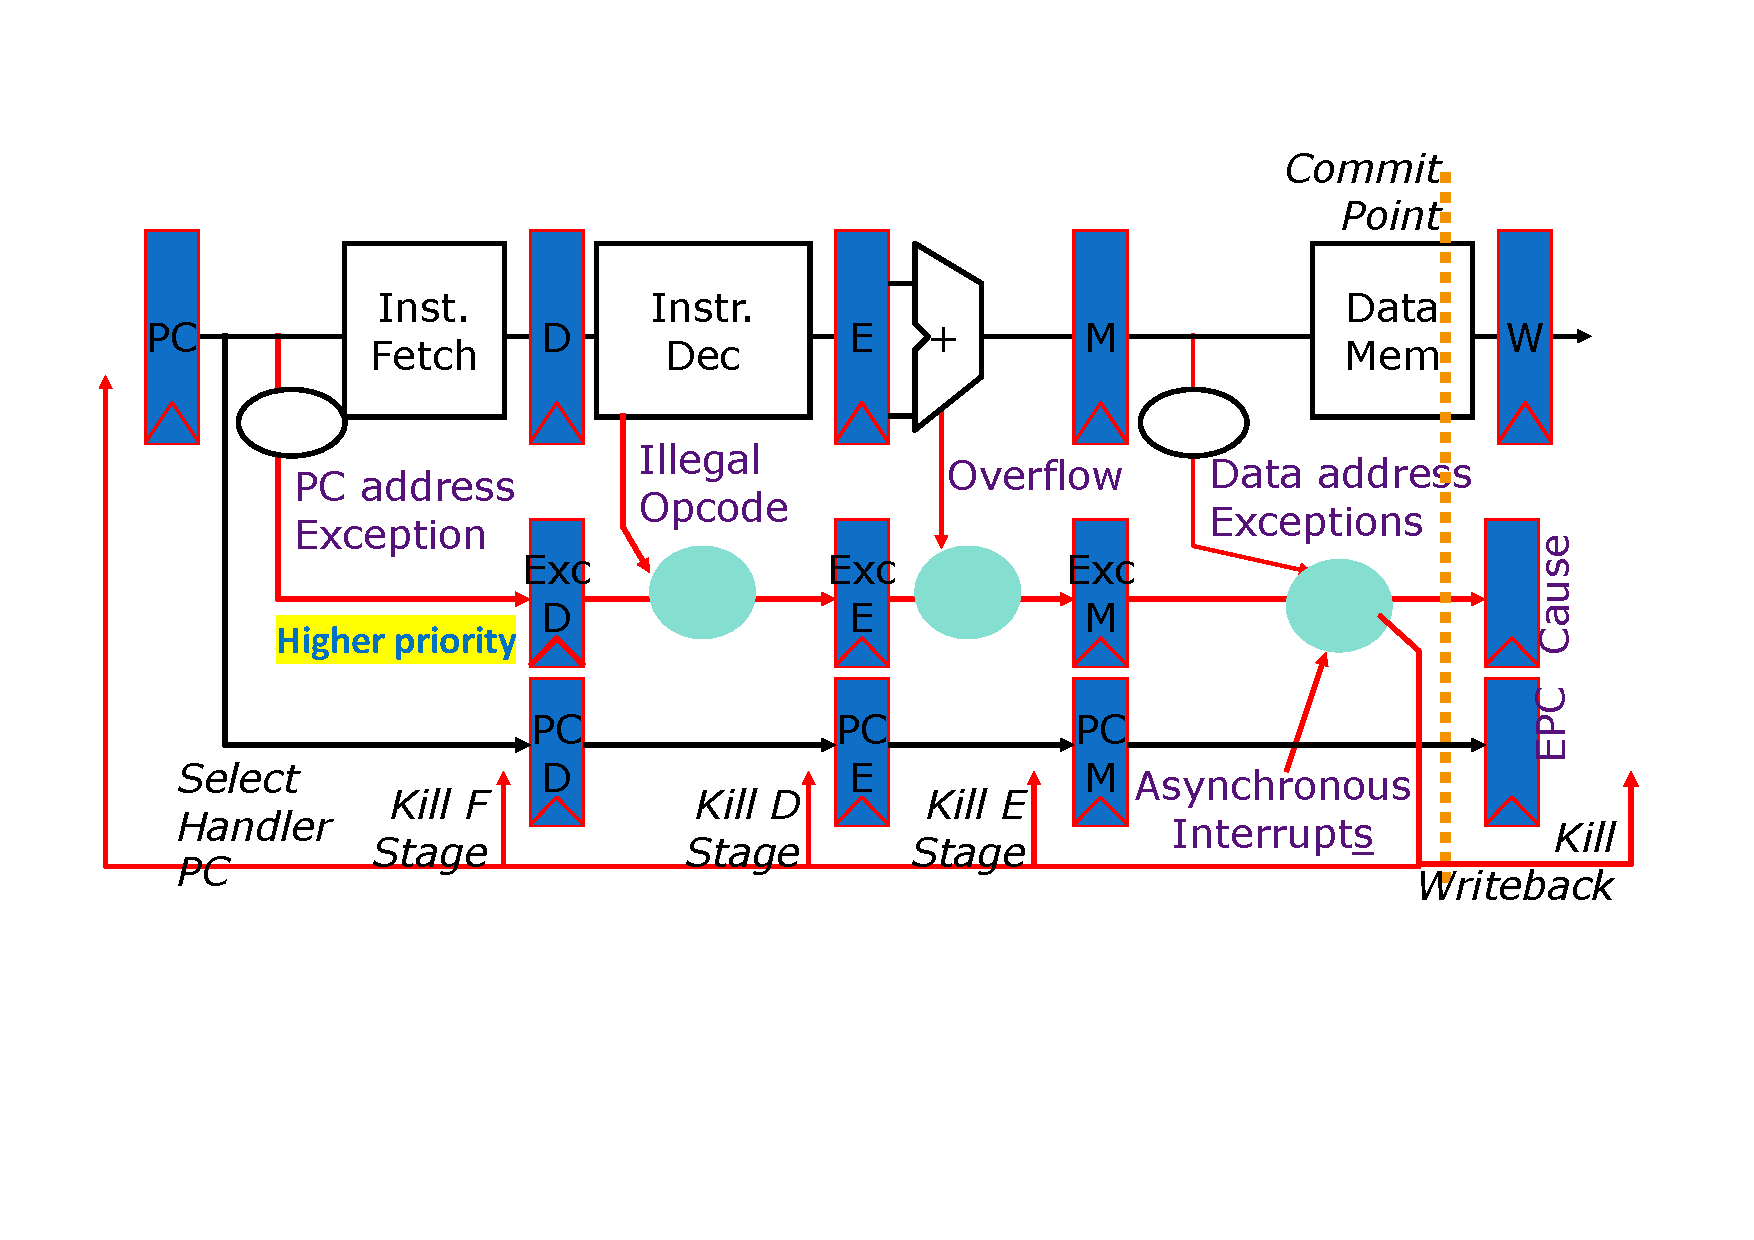
\includegraphics[width=\textwidth]{img/exceptions-in-the-5-stage-pipeline-5.pdf}
    \caption{This is how we solve the out-of-order problem in a pipeline architecture.}
\end{figure}